\documentclass[10pt,a4paper]{article}
\usepackage{amsmath}
\usepackage{amsfonts}
\usepackage{amssymb}
\usepackage{graphicx}
\usepackage{hyperref}
% \usepackage{tikz}
%\usepackage[backend=bibtex]{biblatex}
% \bibliography{bibita.bib} % or
% \addbibresource{<database>.<extension>}
\author{Cerroni Daniele, Scotti Anna, Zunino Paolo}
\title{Geco Improvements towards Stream - THMC}
\begin{document}
\maketitle
In the first part of this report we give a description 
of the new features of Geco and then, in the 
second part, we use this new version of the code
to investigate the evolution of a simplified sedimentary 
basins during a glaciation cycle.
\section{Software updates}
\begin{description}
	\item[Initial porosity.] Modification of Athy law in the file: \texttt{dati.m}.
		$$
		\phi_n\exp\left(-\frac{z_t -z}{\phi_c}\right) \Rightarrow 
		(\phi_n-\phi_{lim})\exp\left(-\frac{z_t -z}{\phi_c}\right)  + \phi_{lim} 
		$$
	\item[Online print.] At the end of every time step the function 
		\texttt{save\_ online\_ res} is called. This function saves 
		the results (the selected vector) into an xml file 
		locate into \texttt{RESU} folder. These files can be read by 
		paraview during the simulation and are 
		numbered according to the time step iteration counter. The actual time
		of the solution is written into the file. Files already present into 
		the \texttt{RESU} folder are not erased by the simulation.

	\item[Concentration.] The transport of the Total Dissolved Solid 
		(TDS) is described through the mass balance equation 
		which reads:
		\begin{equation}
			\frac{\partial C}{\partial t} + u_s \cdot \nabla C = \nabla
			(D \nabla C)
			\label{}
		\end{equation}
		where $C$ is the volume concentration ($Kg/m^3$) of the TDS.
		The function that assembles the system equation  is Ffick implemented into the file \texttt{Ffick.m}
		and also uses the file \texttt{fick\_system.m}. The diffusivity parameter is defined into the 
		file \texttt{dati.m} according to \cite{bense2008transient}.
		It is worth to notice that this system of is analogous to the one that is built for 
		the energy balance equation. All the functions implemented for the energy balance
		equation have been duplicated and adapted to mass transport equation.


	\item[Constitutive laws.] Fluid viscosity and density are expressed as a function of the 
		temperature and the mass concentration field. These relations, implemented into the file 
		\texttt{Materiali.m},  are :
		\begin{equation}
			\mu=1.002\, 10^{-3} \left( 1+ \alpha_1(T) +\alpha_2(C_M) \right)
		\end{equation}
		and 
		\begin{equation}
			\rho_l =  \rho_0(1+\beta_1(T)+ \beta_2(C_M) )\, .
			\label{consrho}
	\end{equation}
		In these relations the temperature ($T$) is expressed in Kelvin 
		and the Concentration ($C_M$) is the molar concentration defined as
		$n_{TDS}/n_{TOT}$ where $n_{TDS}$ 
		and $n_{TOT}$ are the number of TDS and total moles per liter, respectively.
		According to \cite{bense2008transient,jenkins2011convection}
		$\alpha_1$, $\alpha_2$, $\beta_1$ and $\beta_2$ are defined as:
		\begin{equation}
			\begin{aligned}
				&\alpha_1 = 0 \\		
				&\alpha_2 =       0.4819 \left(   \frac{C_M}{55+C_M} \right) 
				+ 0.2774 \left(   \frac{C_M}{55+C_M} \right)^2 
				+ 0.7814 \left(   \frac{C_M}{55+C_M} \right)^3\\		
				&\beta_1  = - 2.07e^{-4}(T-290) \\		
				&\beta_2  =\frac{1e^2}{\rho_0}\left(   \frac{C_M}{55+C_M} \right) \,.\\		
			\end{aligned}
		\end{equation}

	\item[Convergence criterion.] The stopping criterion for 
		the Newton iterations cycle take into
		account also the residual of mass 
		concentration equation. 
		The cycle ends when both the variation of the norm of the displacement 
		and the concentration field is smaller than a given tolerance.  


	\item [Adaptive time step.] The computational time step can change during the simulation.
		This variation is driven by the number of 
		Newton iterations done during a cycle. Let us introduce $n_{max}$ and $n_k$ as the 
		maximum number of newton iterations
		and the number of iterations  done on the $k$ time iteration. 
		In the following time iteration the time step ($\Delta t _{k+1}$) is 
		evaluated according to
		\begin{equation}
			\Delta t _{k+1}=\left\{
				\begin{aligned}
					2 \Delta t _{k} \qquad & n_k<0.2n_{max}\\
					\Delta t _{k} \qquad & 0.2n_{max}<n_k< 0.6n_{max}\\
					0.1\Delta t _{k}  \qquad & n_k>0.6n_{max}
				\end{aligned}
				\right.
			\end{equation}

		\item [Frozen model.] The glaciation model proposed in the final report
			\cite{steam_fp} is now implemented.
			The residual liquid fraction in 
			the computational cell is defied by $\theta_l =S_i \phi_i$ where 
			$S_i$ is defined as:
			\begin{equation}
				S_i=\left\{
					\begin{aligned}
						&1 \quad & T > T_L \,,\\
						&(1-S_{lres})\exp\left[ - \left( \frac{T-T_L}{w}\right)^2 \right] +S_{lres} \quad & T_L> T > T_{lres}\,,\\
						&S_{lres}  \quad &  T < T_{lres}\,,
					\end{aligned}
					\right.
					\label{iceage}
				\end{equation}
				and is implemented into the file \texttt{Materiali.m}.
				Subsequent modifications in the rest of the code are:
				\begin{itemize}
					\item Darcy equations 
						\begin{equation}
							\begin{aligned}
								& \mathbf{u}_d=\frac{1}{\theta_l\mu_l}\mathbf{K}(\phi)k_r(S_i)(\nabla p + \rho_lg) \, ,\\
								& \frac{\partial \theta_l \rho_l}{\partial t} + \nabla \cdot \theta_l \rho_l\mathbf{u}_l = \rho_l Q_l \,.
							\end{aligned}
							\label{}
						\end{equation}
						These modifications are implemented into the file 
						\texttt{Darcy\_system.m}, while $k_r(S_i)$ is implemented in
						\texttt{dati.m}.
					\item Jacobian of the Darcy equation, the term 
						$\frac{\partial \mathbf{K}}{\partial \phi}$ becomes
						\begin{equation}
							\frac{\partial }{\partial \phi }\left( \frac{\mathbf{K}k_r(S_i)}{\theta_l\mu_l} \right)=
							\left( \frac{k_r(S_i)}{\theta_l\mu_l} \right) \frac{\partial \mathbf{K}}{\partial \phi } 
							-\left( \frac{\mathbf{K}k_r(S_i)}{\theta_l\mu_l\phi\
							} \right)\,.
						\end{equation}
						These modifications are implemented into the file \texttt{JJdarcy.m}.
					\item Energy balance equation becomes
						\begin{equation}
							\frac{\partial T}{\partial t }\left( c\rho + L_f\rho_l \frac{\partial \theta_l}{\partial T } 
							\right)+
							c_l\rho_l\mathbf{u}_l \cdot \nabla T = \nabla \cdot \Lambda \nabla T +Q_h \,.
						\end{equation}
						These modifications are implemented into the file \texttt{Fourier\_system.m}, while the 
						constitutive equations that take into account temperature and concentration 
						dependencies are implemented in
						\texttt{dati.m}.
					\item Mass concentration equation balance equation becomes
						\begin{equation}
							\theta_l\frac{\partial C}{\partial t }	+
							\theta_l\mathbf{u}_l \cdot \nabla C = \nabla \cdot \theta_l D \nabla 
							C \,.
						\end{equation}
						These modifications are implemented into the file \texttt{fick\_system.m}, while the 
						constitutive equations that take into account temperature and concentration 
						dependencies are implemented in
						\texttt{dati.m}.

				\end{itemize}
			\item [Time varying inlet temperature.] Top temperature can vary during time. 
				This function is implemented into the file \texttt{Temp\_sea.m}.

			\item[Frame of reference.] The reference point of 
				the domain or, in other words, 
				the zero level of the mono-dimensional 
				coordinate is the deepest point of the domain while
				in the previous version the reference point was the 
				interface between the sea and the basin.
				In order to change the position of the reference point 
				we just translate the domain when the solution is printed into 
				the xml format. Let $\mathbf{z}(\Omega_{old})$ and 
				$\mathbf{z}(\Omega_{new})$ be the coordinate of the domain in the previous 
				and in the modified frame of reference, the relation that links
				the two frameworks is 
				\begin{equation}
					\mathbf{z}(\Omega_{new})=\mathbf{z}(\Omega_{old}) -h_{sea} -z_1(\Omega_{old})\,,
					\label{}
				\end{equation}
				where $h_{sea}$ is the actual height of the sea and $z_1(\Omega_{old}$ is the 
				coordinate of the deepest point of the domain into the old frame of reference
		\end{description}

	
		
		%	(\href{https://danycerr@bitbucket.org/danycerr/geco.git}{https://danycerr@bitbucket.org/danycerr/geco.git}) 
\section{Numerical Results}
%%%%%%%%%%%%%%%%%%%%%%%%%%%%%%%%%%%%%%%%%%%%%%%%%%%%%%%%%%%%%%%%%%%%%%%%%%%%%%%%%%%%%%%%%%
\begin{figure}[htb]
	\centering
	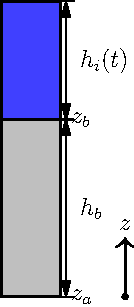
\includegraphics[width=0.2\textwidth]{figure/test_case}
	\caption{Schematic of the sedimentary basin. $h_b$ is the height
	of the sedimentary basins while $h_i$ is the height of the ice sheet above the basins.
In the right lower part of the figure we show the zero value for 
the mono-dimensional coordinate}
	\label{fig:dom}
\end{figure}
%%%%%%%%%%%%%%%%%%%%%%%%%%%%%%%%%%%%%%%%%%%%%%%%%%%%%%%%%%%%%%%%%%%%%%%%%%%%%%%%%%%%%%%%%%%
\begin{figure}[htb]
	\centering
	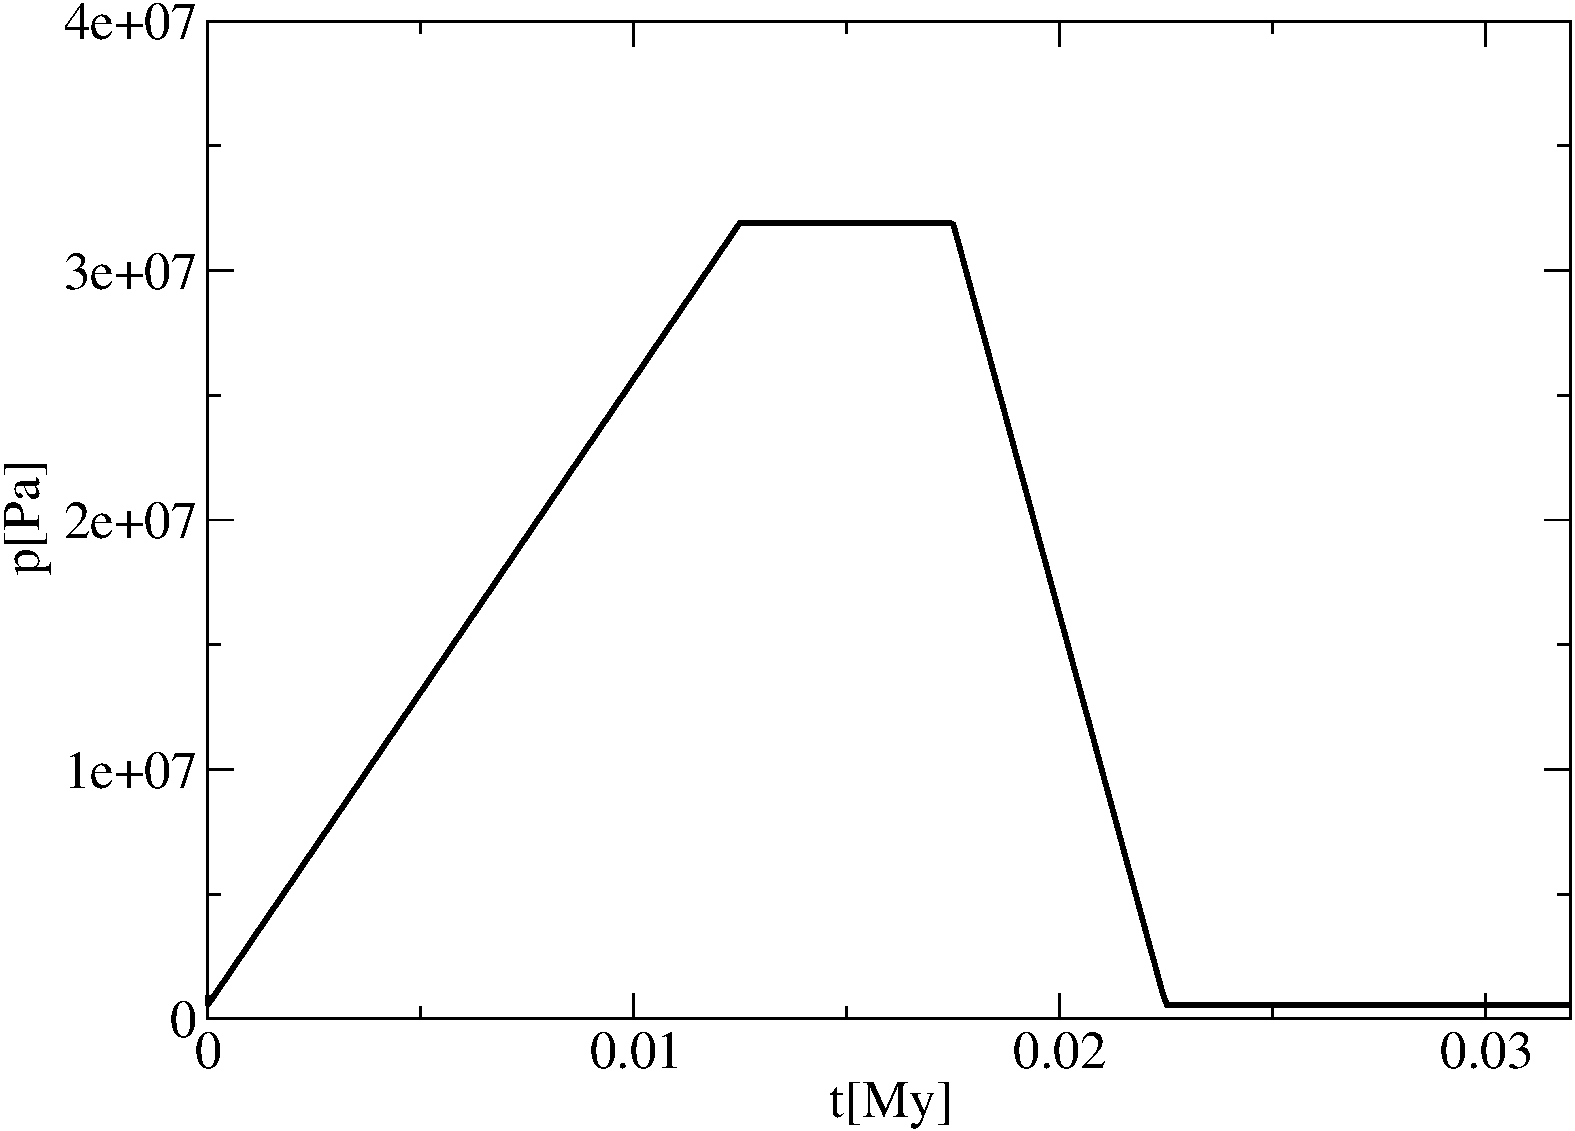
\includegraphics[width=0.6\textwidth]{figure/top_pres}
	\caption{ Pressure on top point of the computational domain over time.}
	\label{fig:pot}
\end{figure}
%%%%%%%%%%%%%%%%%%%%%%%%%%%%%%%%%%%%%%%%%%%%%%%%%%%%%%%%%%%%%%%%%%%%%%%%%%%%%%%%%%%%%%%%%%
%%%%%%%%%%%%%%%%%%%%%%%%%%%%%%%%%%%%%%%%%%%%%%%%%%%%%%%%%%%%%%%%%%%%%%%%%%%%%%%%%%%%%%%%%%%%
\begin{figure}[!htb]
	\centering
	\includegraphics[width=0.8\textwidth]{figure/axialice}
	\includegraphics[width=0.8\textwidth]{figure/axialc}
	\caption{ On the top residual liquid fraction $\theta_l$ at 
		different time steps. On the bottom concentration of TDS 
		at different time steps. $t_a$, 
		$t_b$, $t_c$, $t_d$, $t_e$ and  $t_f$ are
		$0$, $10^-{4}$, $0.2$, $9.5$, $15.5$, $19.7$ and $30 Ky$.	
	}
	\label{fig:res}
\end{figure}
%%%%%%%%%%%%%%%%%%%%%%%%%%%%%%%%%%%%%%%%%%%%%%%%%%%%%%%%%%%%%%%%%%%%%%%%%%%%%%%%%%%%%%%%%%%%%
\begin{figure}[!htb]
	\centering
	\includegraphics[width=0.81\textwidth]{figure/toppoint_all} \hfill
	\includegraphics[width=0.79\textwidth]{figure/toptemp}
	\caption{On the top, darcy velocity in the top node of the 
		domain over time in the test case A, B and C.
		On the bottom, temperature in the top cell
		of the domain over time in the test case A, B and
		C$\equiv$A.
	}
	\label{fig:rescomp}
\end{figure}
%%%%%%%%%%%%%%%%%%%%%%%%%%%%%%%%%%%%%%%%%%%%%%%%%%%%%%%%%%%%%%%%%%%%%%%%%%%%%%%%%%%%%%%%%%
%%%%%%%%%%%%%%%%%%%%%%%%%%%%%%%%%%%%%%%%%%%%%%%%%%%%%%%%%%%%%%%%%%%%%%%%%%%%%%%%%%%%%%%%%%
%%%%%%%%%%%%%%%%%%%%%%%%%%%%%%%%%%%%%%%%%%%%%%%%%%%%%%%%%%%%%%%%%%%%%%%%%%%%%%%%%%%%%%%%%
In this Section we firstly describe the investigated problem 
and then we show some preliminary results.
The test case that we consider is the one proposed in \cite{bense2008transient}, 
it includes time varying altitude of the glacier and a time 
dependent temperature field at the		basin  glacier interface.
In \cite{bense2008transient} the compaction of the basin is not investigated 
and no freezing model is considered therefore in our test 
we consider the ice formation into the basin according to 
the model proposed in 
\cite{steam_fp,jenkins2011convection}.
The constitutive parameters
 such as thermal expansion coefficient, thermal diffusivity, density, etc.
 used in this test, are the ones typical for sedimentary basins 
 and commonly used in literature \cite{jenkins2011convection,bense2008transient}.
 The geometry of the idealized sedimentary basin
considered is representative of an intercratonic 
sag basin. In Figure \ref{fig:dom} the schematic of the sedimentary basin
together with the frame of 
reference of the simulation is shown. $h_b$ is the height
of the sedimentary basins while $h_i$ is
the height of the ice sheet above the basins.
The basin has an initial depth ($h_b$) of
$5000 m$  which dimensions are
comparable to that of the Michigan 
or Illinois basins \cite{bense2008transient}.
The time period considered is $32 Ky$ and during
this time the ice sheet above the basin varies according to
\begin{equation}
				h_i(t)=\left\{
				\begin{aligned}
					& \frac{h_M-h_m}{t_1}t + h_m \qquad & t<t_1 \,, \\
					& h_M \qquad & t_1<t<t_2 \,,\\
					& \frac{h_M-h_m}{t_2-t_3}(t-t3) + h_m \qquad & t_2<t<t_3\,,\\
					& h_m \qquad & t_3<t<t_4 \,,\\
				\end{aligned}
				\right.
\end{equation}
where $t_1$, $t_2$, $t_3$ and $t_4$ are 
$ 12.5 Ky $, $ 17.5 Ky $, $ 22.5 Ky $ and $ 32.5 Ky $, respectively. 
$h_M$ and $h_m$ are the maximum and the minimum
height of ice sheet above the basin and are equal to
$3200m$ and $0m$, respectively.
The boundary conditions for the energy balance equation 
are non-homogeneous Dirichlet and homogeneous
Neuman on the top and the bottom part 
of the domain, respectively.
The temperature field in the top of the domain (ice basin interface)
is not constant during the simulation and is defined by 
\begin{equation}
	T_{top}(t)=\left\{
				\begin{aligned}
					& \frac{T_M}{t_1}t  \qquad & t<t_1 \,, \\
					& T_M\frac{t-t_2}{t_1-t_2} \qquad & t_1<t<t_2\,,\\
				\end{aligned}
				\right.
\end{equation}
where $T_M$ is $263 \, K$.
The residual liquid fraction ($\theta_l$ ) 
which does not freeze is evaluated through the relation
\begin{equation}
	\theta_l=S_i\phi_i
\end{equation}
where $S_i$ is defined by eq. (\ref{iceage}).
The initial concentration field of the TDS is a linear profile 
between the top and the bottom value, $0.1$ and $0.25 \,,g/l$, respectively.
The boundary condition for for the mass transport problem are
homogeneous Dirichlet and homogeneous Neuman in the top 
and the bottom of the basins, respectively.
In Figure \ref{fig:pot} the pressure in the highest element 
of the computational domain over time is shown. We can see that 
because of the variation of the 
thickness of the ice sheet the hydro-static 
load in the inlet region of the basin varies over time.
In the top part of Figure \ref{fig:res} the residual 
liquid fraction ($theta_l$) in the domain at different
time steps is shown together with the concentration
of the TDS on the bottom. We can observe that when the 
temperature reach the freezing interval, the residual liquid part 
suddenly reduces to zero. 
The ice presence effectively modifies 
the physical and the mechanical properties of
the system. In order to show highlight the importance 
of the ice formation we consider three test case, the 
case A is the reference case in which we consider both the 
formation of ice and the dependency of the physical 
properties from the temperature field. 
In the case B we neglect the ice formation
by assuming $S_{lres}=1$ in eq. (\ref{iceage}) while
in the case C we neglet the effect of the temperature
field in the fluid density by considering $\beta_1=0$ into eq.
(\ref{consrho}).
In the top part of Figure \ref{fig:rescomp} the module of 
the filtration 
velocity in the highest point of the domain is shown for the 
different test cases A,B and C. 
We can notice that in all cases we obtain 
different results. The case B, where 
we neglect the ice formation, 
leads to a faster dynamics of the basins while 
in the case C the Darcy velocity is much smaller with 
respect to the one evaluated in the reference case (A). 
In the bottom part of Figure \ref{fig:rescomp} the 
temperature field in the top cell of the domain is shown.
In this Figure the test cases A and C produce the 
same results. We can notice that neglecting the ice formation,
case B, leads to the evaluation of a temperature 
field different from the one obtained in the other cases.
These differences are mostly due to the different physical 
properties of the ice that are not taken into account 
in the case B.

\section{Conclusion}
In this report we have shown the new features 
of the current version of Geco. 
These  new features allows 
to study the evolution of a sedimentary basin 
during a glaciation cycle taking into account
the formation of ice inside the basin. Moreover
we have introduced the mass transport 
equation that can be used to study the 
transport of a non reactive species, such 
as TDS, inside the porous domain.


In the second part of the report 
we have shown preliminary results obtained 
performing a test case taken from literature. 
In particular we have shown that neglecting 
any part of the complete mathematical model leads to 
a difference in the obtained results.


%%%%%%%%%%%%%%%%%%%%%%%%%%%%%%%%%%%%%%%%%%%%%%%%%%%%%%%%%%%%%%%%%%%%%%%%%%%%%%%%%%%%%
		\bibliography{bibita}
		\bibliographystyle{ieee}
%%%%%%%%%%%%%%%%%%%%%%%%%%%%%%%%%%%%%%%%%%%%%%%%%%%%%%%%%%%%%%%%%%%%%%%%%%%%%%%%%%%%%%%%%%
		\end{document}
